\documentclass{beamer}
%\usepackage[margin=1in]{geometry}
\usepackage{amsthm,amsmath,amsfonts,hyperref,graphicx,color,multicol}
\usepackage{enumitem,tikz}

%%%%%%%%%%
%Beamer Template Customization
%%%%%%%%%%
\setbeamertemplate{navigation symbols}{}
\setbeamertemplate{theorems}[ams style]
\setbeamertemplate{blocks}[rounded]

\definecolor{Blu}{RGB}{43,62,133} % UWEC Blue
\setbeamercolor{structure}{fg=Blu} % Titles

%Unnumbered footnotes:
\newcommand{\blfootnote}[1]{%
	\begingroup
	\renewcommand\thefootnote{}\footnote{#1}%
	\addtocounter{footnote}{-1}%
	\endgroup
}


%%%%%%%%%%
%Custom Commands
%%%%%%%%%%
\newcommand{\R}{\mathbf{R}}
\newcommand{\veca}{\vec{a}}
\newcommand{\vecb}{\vec{b}}
\newcommand{\vece}{\vec{e}}
\newcommand{\vecu}{\vec{u}}
\newcommand{\vecv}{\vec{v}}
\newcommand{\vecw}{\vec{w}}
\newcommand{\vecx}{\vec{x}}
\newcommand{\zerovector}{\vec{0}}

\newcommand{\ds}{\displaystyle}

\newcommand{\fn}{\insertframenumber}

\newcommand{\rank}{\operatorname{rank}}
\newcommand{\adj}{\operatorname{adj}}

\newcommand{\blank}[1]{\underline{\hspace*{#1}}}


%%%%%%%%%%
%Custom Theorem Environments
%%%%%%%%%%
\theoremstyle{definition}
\newtheorem{exercise}{Exercise}
\newtheorem{question}[exercise]{Question}
\newtheorem*{defn}{Definition}
\newtheorem*{exa}{Example}
\newtheorem*{disc}{Group Discussion}
\newtheorem*{nb}{Note}
\newtheorem*{recall}{Recall}
\renewcommand{\emph}[1]{{\color{blue}\texttt{#1}}}

\definecolor{Gold}{RGB}{237, 172, 26}
%Statement block
\newenvironment{statementblock}[1]{%
	\setbeamercolor{block body}{bg=Gold!20}
	\setbeamercolor{block title}{bg=Gold}
	\begin{block}{\textbf{#1.}}}{\end{block}}





\begin{document}
	\title{Math 324: Linear Algebra}
	\subtitle{Section 4.2: Abstract Vector Spaces}
	\author{Mckenzie West}
	\date{Last Updated: \today}
\begin{frame}
\maketitle
\end{frame}

\begin{frame}{\insertframenumber}
	\begin{block}{\textbf{Last Time.}}
	\begin{itemize}[label=--]
		\item Vectors in $\R^2$
		\item Vectors in $\R^n$
	\end{itemize}
	\end{block}
	\begin{block}{\textbf{Today.}}
		\begin{itemize}[label=--]
			\item Abstract Vector Spaces
			\item Important Vector Spaces
			\item Proving Something is not a Vector Space
		\end{itemize}
	\end{block}
\end{frame}
\begin{frame}{\fn}
	\begin{defn}
		Let $V$ be a set with two operations, \emph{vector addition} and \emph{scalar multiplication} (by real numbers, $\R$).
		
		We call $V$ a \emph{vector space} if the following hold for all $\vec u,\vec v,\vec w\in V$ and all $c,d\in\R$:
			\begin{enumerate}[label=\textbf{\arabic*.}]
				\item $\vec{u}+\vec v\in V$\hfill \emph{(additive closure)}
				\item $\vec u+\vec v=\vec v+\vec u$\hfill \emph{(commutativity of addition)}
				\item $(\vec u +\vec v)+\vec w = \vec u+(\vec v + \vec w)$\hfill\emph{(associativity of addition)}
				\item $\exists\ \vec 0\in V$ s.t. $\vec u +\vec 0= \vec u$\hfill\emph{(additive identity)}
				\item $\exists\ (-\vec u)\in V$ s.t. $\vec u+(-\vec u)=\vec 0$\hfill\emph{(additive inverse)}
				\item $c\vec u\in V$ \hfill\emph{(scalar closure)}
				\item $c(\vec u+\vec v)=c\vec u+c\vec v$\hfill\emph{(distributivity)}
				\item $(c+d)\vec u = c\vec u + d\vec u$\hfill\emph{(distributivity)}
				\item $c(d\vec u)=(cd)\vec u$\hfill \hfill\emph{(associativity of scalars)}
				\item $1(\vec u)=\vec u$\hfill \emph{(multiplicative identity)}
			\end{enumerate}
	\end{defn}
\end{frame}
\begin{frame}{\fn}
	\begin{exa}
		For all integers $n$, the set of $n$-dimensional vectors, $\R^n$, is a vector space with the standard operations by Theorem 4.2.
	\end{exa}
	\begin{exa}
		For all integers $m$ and $n$, the collection of $m\times n$ matrices, denoted $M_{m,n}$, with the standard operations is a vector space by Theorems 2.1 and 2.2.
	\end{exa}
\end{frame}
\begin{frame}{\fn}
	\begin{exercise}
		Show that $\{(x,x)\ :\ x\in \R\}$ (read this as, \textit{the collection of ordered pairs $(x,x)$ such that $x$ is in $\R$}) is a vector space with the standard operations in $\R^2$ by verifying all 10 axioms of a vector space.
	\end{exercise}
	\begin{exercise}
		Show that $P_2$, the set of polynomial of degree at most $2$, along with the zero polynomial, $p(x)=0$, is a vector space.

		\begin{nb}
			Formally the degree of the polynomial $p(x)$ tells us the maximum possible values of $x$ satisfy $p(x)=0$. And so the zero polynomial either does not have a degree or is considered to have degree $\infty$.
		\end{nb}
	\end{exercise}
\end{frame}
\begin{frame}{\fn}
	\begin{exercise}
		Let $V$ be the collection of all continuous functions $f(x)$ such that $f(0)=0$.  The sum of two functions $f$ and $g$ is the function $f+g$ where $(f+g)(x):= f(x)+g(x)$.  The scalar multiple of the function $f$ by $c$ is the function $cf$ where $(cf)(x):= c(f(x))$.
		
		Is $V$ a vector space?  
		
		(Don't get too far into the calculus, but do make sure to convince yourself of the additive and scalar closure properties.)
	\end{exercise}
	\begin{exercise}
		Can you think of any other vector spaces?
	\end{exercise}
\end{frame}
\begin{frame}{\fn}
	\begin{block}{\textbf{Important Vector Spaces with Notation}}
		\begin{tabular}{rcl}
			$\R$&=&set of all real numbers\\
			$\R^n$&=&set of all $n$-tuples, as described in the previous class\\
			$C(-\infty,\infty)$&=&set of all continuous functions with domain $\R$\\
			$C[a,b]$&=&set of all continuous functions defined on $[a,b]$\\
			$P$&=&set of all polynomials\\
			$P_n$&=&set of all polynomials of degree $\leq n$\\ &&along with the zero polynomial\\
			$M_{m,n}$&=&set of all $m\times n$ matrices\\
			$M_n$&=&set of all $n\times n$ matrices
		\end{tabular}
	\end{block}
\end{frame}
\begin{frame}{\fn}
	\begin{exercise}
	 	Watch: Several of the videos linked in the Canvas question. These videos complete the proof that the following set and operations form a vector space.\\
	 	Show that $V=\{(x,y)\ :\ x,y\in\R \text{ and }y> 0\}$ is a vector space with the operations:
	 	$$\begin{array}{rcl}	
	 		\text{Addition: \hspace*{.35in}} (x_1,y_1)\oplus (x_2,y_2)&=&(x_1+x_2,y_1y_2)\\
	 		\text{Scalar Multiplication: \hspace*{.1in}} c*(x,y)&=&(cx,y^c)
	 		\end{array}$$
	\end{exercise}
	\begin{nb}
		Sometimes we use different notation for addition, eg. $\oplus$, and scalar multiplication, eg. $*$, to distinguish it from the standard operations.
	\end{nb}
\end{frame}

\begin{frame}{\fn}
	\begin{block}{\textbf{Brain Break.}}
		What is your favorite candy?
		\begin{center}
			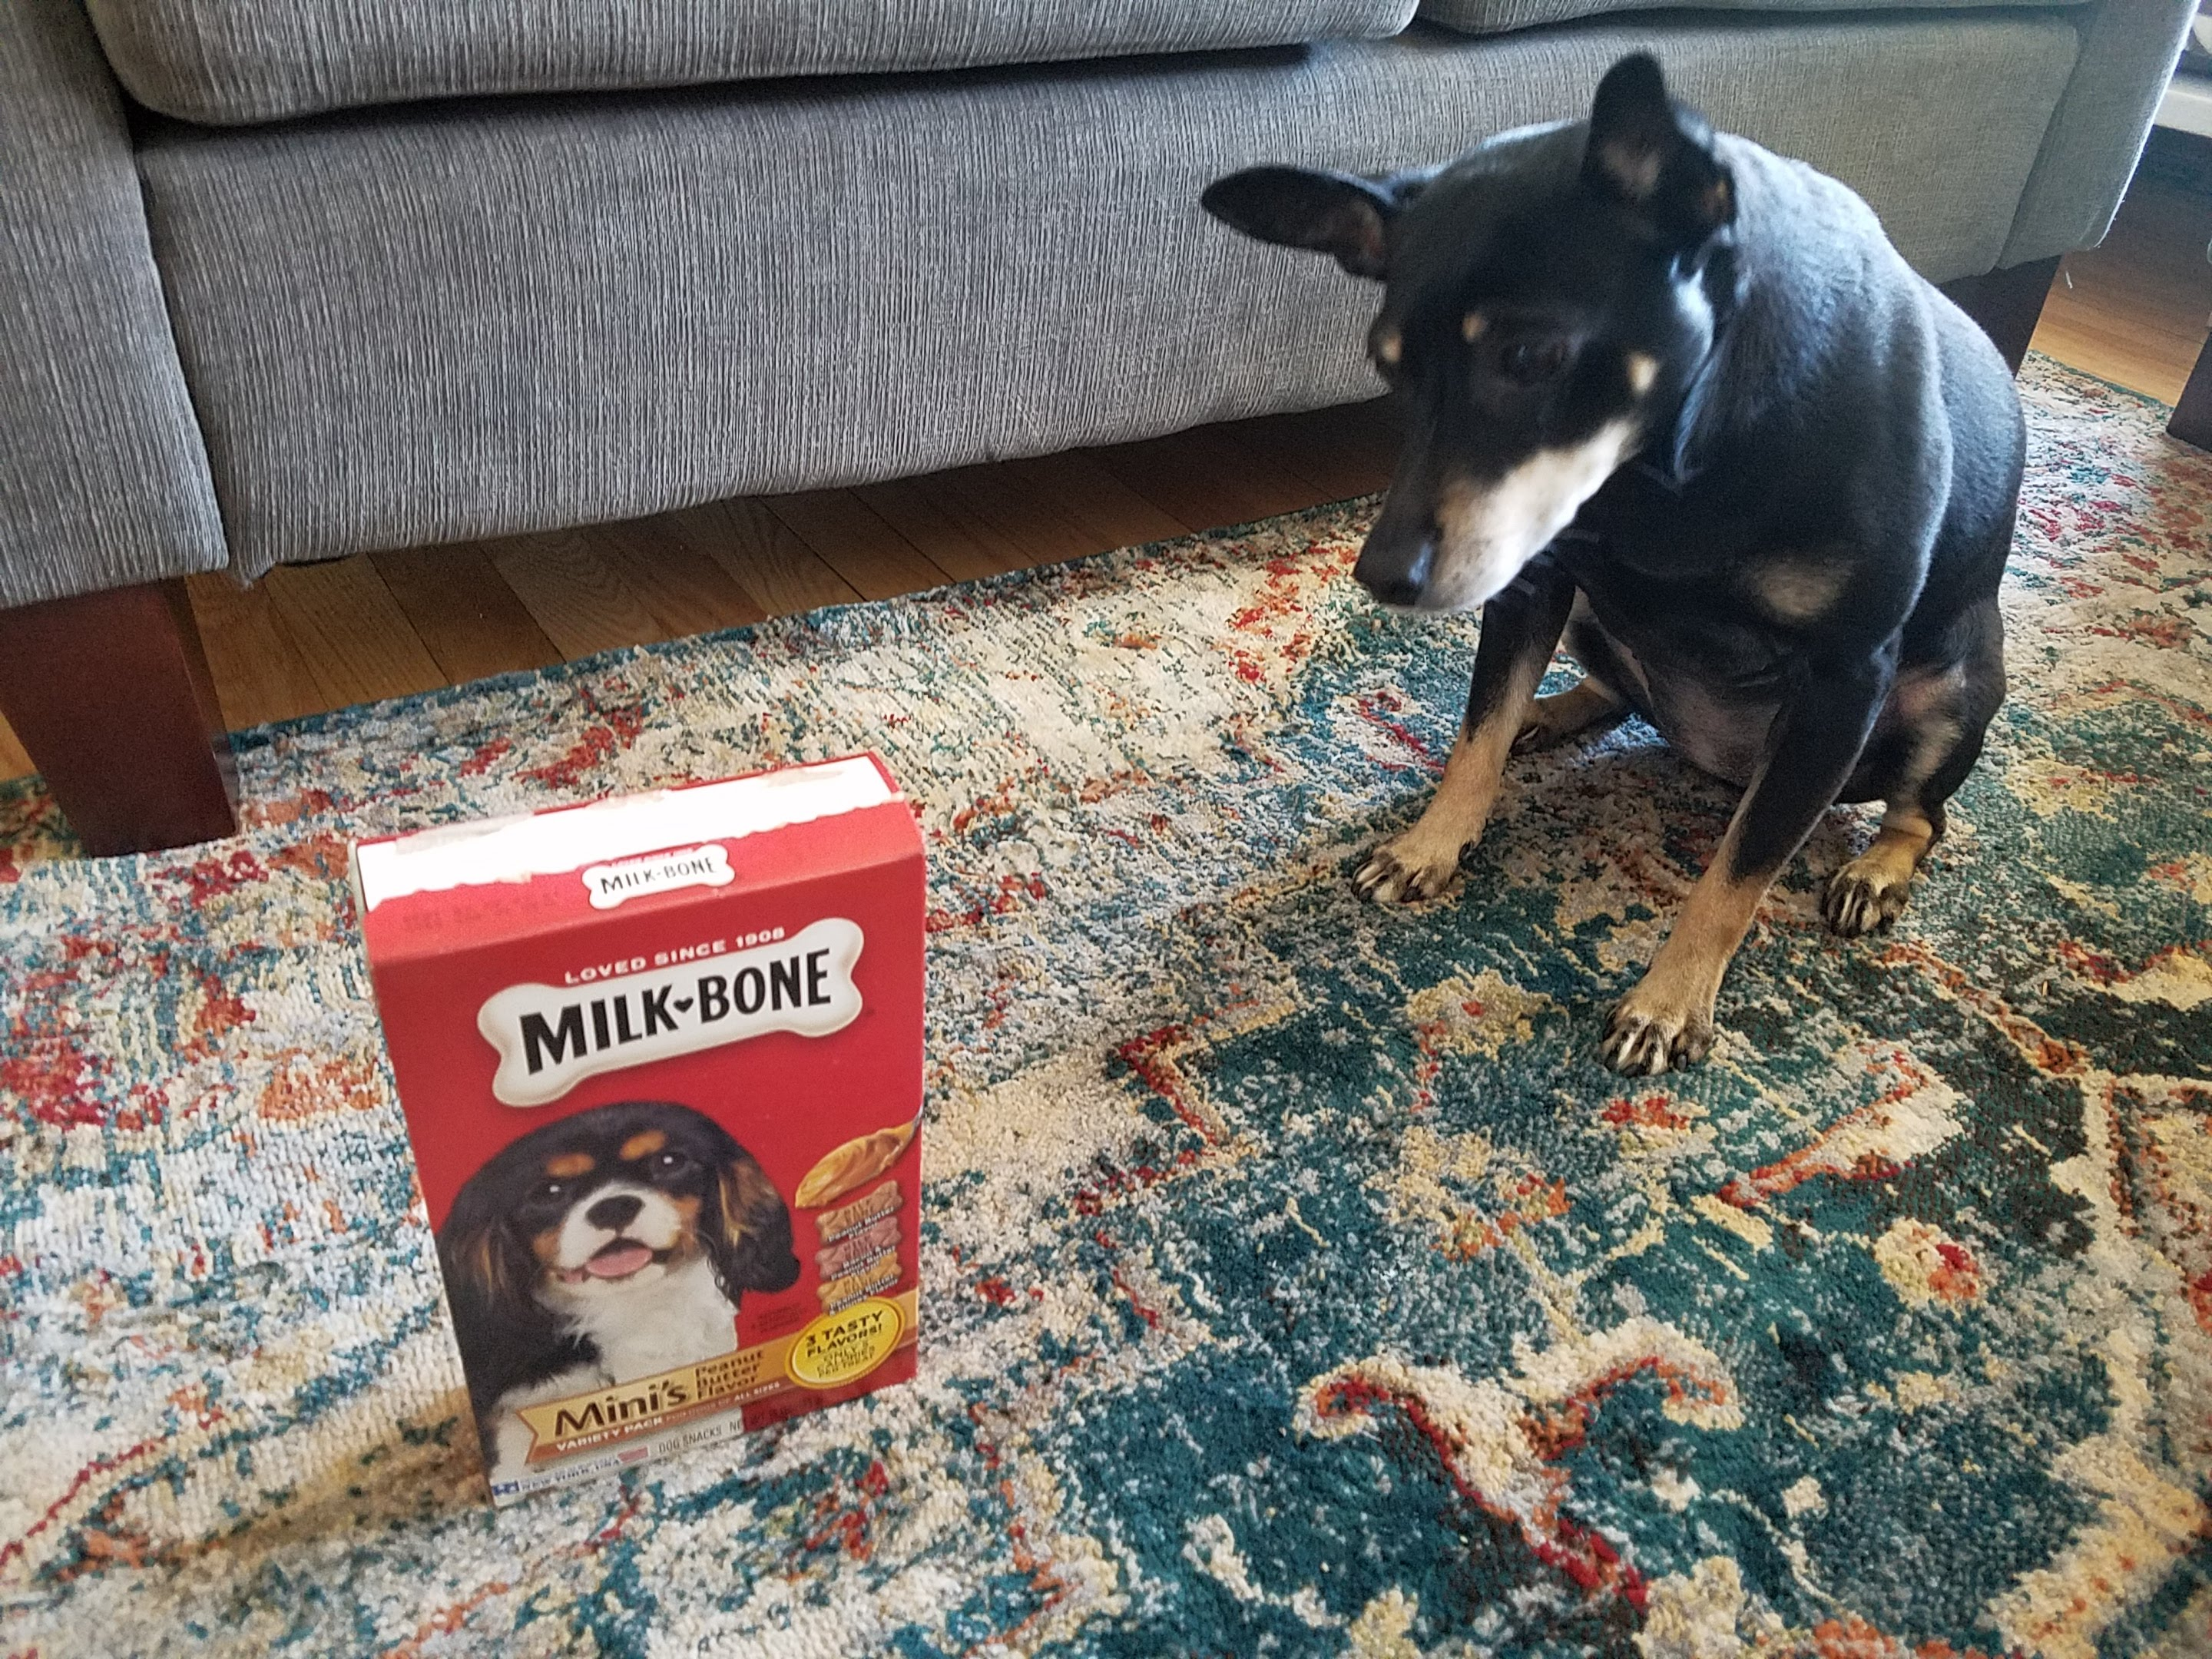
\includegraphics[width=2in]{../images/treat_Pepper}
		\end{center}
		I am pretty sure Pepper's favorite snack food is peanut butter.
	\end{block}
\end{frame}
\begin{frame}{\fn}
	\begin{exa}
		To show that something is not a vector space, we simply have to give an example where one of the axioms fails.  For example the collection $S$ of all continuous functions $f(x)$ such that $f(0)=1$ is not a vector space because:
		
			\begin{center}
				\begin{minipage}{.8\textwidth}
					If $f(x)=1$ then $(2f)(0)=2\neq1$, so $2f\not\in S $. Thus $S$ is not closed under scaling.\hfill\qedsymbol
				\end{minipage}
			\end{center} 
	\end{exa}
	\begin{exercise}
		What other properties does the set from the previous example fail?
	\end{exercise}
\end{frame}
\begin{frame}{\fn}
	\begin{exercise}
		Consider the set with $V=\R^2$ where we have the standard definition of addition but scalar multiplication is defined via:\[c(x,y)=(0,cy).\]
		
		Which axioms does this set/operations fail?
	\end{exercise}
\end{frame}
\begin{frame}{\fn}
	\begin{exercise}
		Which of the following are vector spaces? (Hint: None are, why not?)
	\begin{enumerate}[label=(\alph*)]
		%\item The set $\{(x,0)\ :\ x\in\R\}$ with the standard operation on $\R^2$.
		\item The set $\{(x,y)\ :\ x,y\in\R\text{ and }x,y\geq0\}$ with the standard operations on $\R^2$.
		%\item The set $D_n$ of $n\times n$ diagonal matrices with the standard operation on $M_n$.
		%\item The set $U_n$ of $n\times n$ upper triangular matrices with the standard operations on $M_n$.
		\item The set of $2\times 2$ matrices of the form $\begin{bmatrix}1&b\\c&1\end{bmatrix}$ with the standard operations on $M_2$.
		\item The set $2\times 2$ nonsingular matrices with the standard operations on $M_2$.
		\item The set of degree exactly 2 polynomials.
	\end{enumerate}
	\end{exercise}
\end{frame}
%\begin{frame}{\fn}
%	\begin{exercise}
%		Solve the homogeneous system of equations with coefficient matrix \[A=\begin{bmatrix}1&1&1\\2&2&2\\3&3&3\end{bmatrix}.\]
%	
%	Is the set of solutions to this system a vector space with standard operations from $\R^3$?
%	\end{exercise}
%	\begin{exercise}
%		Let $A=\begin{bmatrix}1&2\\3&6\end{bmatrix}$ and $\vec b=\begin{bmatrix}-1\\-3\end{bmatrix}$.  Is the set of solutions to the system $A\vec x=\vec b$ a vector space with the standard operations in $\R^2$?
%	\end{exercise}
%\end{frame}
%\begin{frame}{\fn}
%	\begin{exercise}
%		Let $A$ be any $2\times 2$ matrix.  Prove that the set of solutions to the homogeneous system $A\vec x=\vec 0$ is a vector space.
%	\end{exercise}
%	\begin{exercise}
%		Let $A$ be any $2\times 2$ matrix.  Prove that the set of solutions to the inhomogeneous system $A\vec x=\vec b$ where $\vec b\neq \vec 0$ is not a vector space.
%	\end{exercise}
%\end{frame}
\begin{frame}{\fn}
	\begin{exercise}[Challenge - Optional]
		Rather than the standard definitions of addition and scalar multiplication on $\R^2$ use the given definition.  Which operations produce a vector space on $\R^2$?  Justify your answers.
		\begin{enumerate}[label=(\alph*)]\setlength{\itemsep}{.15in}
			\item $\begin{array}{rcl}(x_1,y_1)+(x_2,y_2)&=&(x_1,y_2)\\c(x_1,y_1)&=&(cx_1,cy_1)\end{array}$
			\item $\begin{array}{rcl}(x_1,y_1)+(x_2,y_2)&=&(y_1+y_2,x_1+x_2)\\c(x_1,y_1)&=&(cx_1,cy_1)\end{array}$
%			\item $\begin{array}{rcl}(x_1,y_1)+(x_2,y_2)&=&(x_1+x_2,y_1+y_2)\\c(x_1,y_1)&=&(c^2x_1,c^2y_1)\end{array}$
%			\item $\begin{array}{rcl}(x_1,y_1)+(x_2,y_2)&=&(x_1x_2,y_1y_2)\\c(x_1,y_1)&=&(cx_1,cy_1)\end{array}$
		\end{enumerate}
	\end{exercise}
\end{frame}
%\begin{frame}{\fn}
%	\begin{statementblock}{Theorem 4.4}
%		Let $\vec v$ be any element of a vector space $V$, and let $c$ be a scalar.  Then the following properties are true.
%		\begin{enumerate}[label=\textbf{\arabic*.}]
%			\item $0\vec v=\vec 0$
%			\item $c\vec 0=\vec 0$
%			\item If $c\vec v=\vec 0$, then $c=0$ or $\vec v=\vec 0$.
%			\item $(-1)\vec v=-\vec v$
%		\end{enumerate}
%	\end{statementblock}
%	\begin{exercise}
%		Verify all four of these results for the goofy vector space from exercise 6: (first remind yourself of what $\zerovector$ and $-\vecv$ were)
%			\begin{quote}
%				$V=\{(x,y)\ :\ x,y\in\R \text{ and }x> 0\}$ with the operations:
%				$$\begin{array}{rcl}	
%				\text{Addition: \hspace*{.35in}} (x_1,y_1)\oplus (x_2,y_2)&=&(x_1x_2,y_1+y_2)\\
%				\text{Scalar Multiplication: \hspace*{.1in}} c*(x,y)&=&(x^c,cy)
%				\end{array}$$
%			\end{quote}
%	\end{exercise}
%\end{frame}
%\begin{frame}{\fn}
%	Just like in the case of $\R^n$ we can consider linear combinations for general vector spaces.
%	\begin{defn}
%		A vector $\vec v$ in a vector space $V$ is a \emph{linear combination} of $\vec u_1,\vec u_2,\dots,\vec u_n\in V$ if there exist scalars $c_1,c_2,\dots,c_n$ such that
%			\[\vec v=c_1\vec u_1+c_2\vec u_2+\cdots+c_n\vec u_n.\]
%	\end{defn}
%	\begin{exa}
%		The polynomial $p(x)=3+x-2x^2$ is a linear combination of $q_1(x)=1+x$, $q_2(x)=1+x^2$, $q_3(x)=1+x+x^2$, and $q_4(x)=x^2$ because \begin{eqnarray*}p(x)&=&3+x-2x^2\\ &=&5(1+x)+2(1+x^2)-4(1+x+x^2)+0x^2\\&=&5q_1(x)+2q_2(x)+(-4)q_3(x)+0q_4(x)\end{eqnarray*}
%	\end{exa}
%\end{frame}
%\begin{frame}{\fn}
%	\begin{exercise}
%			Can the polynomial $p(x)=1-4x+x^2$ be written as a linear combination of $q_1(x)=1+x$ and $q_2(x)=1+x^2$?
%	\end{exercise}
%	\begin{exercise}
%		Describe all of the polynomials can be written as a linear combination of $q_1(x)=1+x$ and $q_2(x)=1+x^2$.
%	\end{exercise}
%\end{frame}
\end{document}

